\section{Simulation Layer}
As shown in the Design section, the Simulation layer is split into generic Runners and multiple simulation Backends.
Building a system that efficiently allowed Runners to be Backend-agnostic and still performance was nontrivial.

\subsection{Runners}
Runners had three major design constraints:
\begin{enumerate}
    \item Runners should be generic with respect to the backends they implement.
    \item The same Runner should have the same interface for each Backend it implements.
    \item Virtual functions should be avoided where possible.
\end{enumerate}
The immediate thought would be to implement a single Runner class, taking a virtual Backend class and uses virtual functions to start each tick.
This would meet (1) by using a virtual Backend interface, and (2) by using exactly the same class for all Backends, but would violate (3) by forcing every Backend to use virtual classes.
Instead, a slightly more complex approach is taken.

Each Runner defines a virtual interface, such as \mintinline{cpp}{IFixedTimeRunner} for the \mintinline{cpp}{FixedTimedRunner}.
A templated implementation class is then instantiated for each compatible backend, such as \mintinline{cpp}{SimFixedTimeRunner<CpuBackend>}, \mintinline{cpp}{SimFixedTimeRunner<CUDABackendV1>}, etc.
Each of these classes implements the virtual interface \mintinline{cpp}{IFixedTimeRunner}, but they call the simulation functions directly as they are templated on the backend type.
This setup meets (1) by using a single templated implementation, (2) by implementing a virtual interface, and (3) by only using the virtual functions where absolutely necessary i.e. on the Runner itself.
This allows the \mintinline{cpp}{FixedTimeRunner} to define a single virtual function \mintinline{cpp}{runForTime(t)} instead of calling a virtual function every simulation tick.

\subsection{Backends}
To allow the generic implementation described above, the Backend typeclass (\cref{fig:TypeclassBackend}) ensures all backends follow a consistent interface.
Five classes implement this typeclass, matching those described in \cref{sec:DesignBackends}:
\begin{itemize}
    \item \mintinline{cpp}{NullSimulation}
    \item \mintinline{cpp}{CPUSimpleSimBackend}
    \item \mintinline{cpp}{CPUOptimizedSimBackend}
    \item \mintinline{cpp}{CPUOptimizedAdaptedSimBackend}
    \item \mintinline{cpp}{CudaBackendV1}
\end{itemize}
Aside from the trivial Null Simulation, these can be split into CPU and CUDA-based backends.

\begin{figure}
    \centering
\begin{cppcode}
typeclass BackendFrame {
    // Must have a constructor that takes an allocator
    BackendFrame(FrameAllocator<MemoryType> allocator);
}
typeclass Backend {
    // Must define a Frame class
    class Frame fits BackendFrame;
    // Must have a constructor
    Backend(std::vector<Frames>, FluidProperties, SimSnapshot);
    
    float findMaxTimestep();
    void tick(float timestep, int targetFrame);
    
    LegacySimDump dumpStateAsLegacy();
    SimSnapshot get_snapshot();
}    
\end{cppcode}
    \caption{Backend typeclass}
    \label{fig:TypeclassBackend}
\end{figure}

\subsubsection{CPU Backends}
Most of the simulation code for these backends has been directly copied from the ACA simulation\cite{modules:aca257submission}.
Some templates and template specializations have been added for the Adapted backend, but for the most part the simulation is unchanged.
The backend classes simply wrap up this code to be compatible with the typeclass.

\subsubsection{CUDA Backend}
\begin{figure}[t]
    \centering
    \begin{subfigure}{0.49\textwidth}
        \begin{minted}{cpp}
template<typename T>
using in_matrix = 
    const T* const __restrict__;

template<typename T>
using out_matrix = 
    T* const __restrict__;
        \end{minted}
        \caption{Matrix templates}
    \end{subfigure}%
    \begin{subfigure}{0.49\textwidth}
        \begin{minted}{cuda}
__global__ void computationKernel(
    CommonParams config,
    in_matrix<float> inputs1,
    in_matrix<int> inputs2,
    
    out_matrix<float> output
);
        \end{minted}
        \caption{A kernel using the matrix templates}
    \end{subfigure}
    \caption{Example of CUDA matrix templates}
    \label{fig:ImplMatrices}
\end{figure}

The CUDA backend is where the bulk of new simulation work has been done.
As stated in the Design section, all simulation code has been ported to CUDA Kernels.
Each of these kernels takes a \mintinline{cpp}{CommonParams} struct as the first argument, containing run-time constants such as the simulation grid size.
To ensure \mintinline{cpp}{const __restrict__} pointers are used wherever possible, all other kernel arguments must be either an \mintinline{cpp}{in_matrix<T>} or an \mintinline{cpp}{out_matrix<T>}.
These templates alias to simple pointers which properly use \mintinline{cpp}{const} and \mintinline{cpp}{__restrict__} (\cref{fig:ImplMatrices}).
Using these enforces that each kernel has clear, distinct inputs and outputs, and that the inputs are read from fast global memory.

The most intensive step in every implementation is the Poisson iterations, which are individually trivial but intensive at scale.
During development the profiler showed large gaps between the individual kernel runs, equivalent to almost 50\% of the runtime.
Each kernel was finishing quicker than the CPU could enqueue a new one, so to solve this a CUDA Graph was employed.
CUDA Graphs consist of a prerecorded set of kernel invocations with constant arguments.
A CUDA Graph was recorded that consisted of 100 Poisson kernels, and this was launched instead of the individual kernels.
This resulted in a 2x speedup in the profiler (see \cref{fig:CudaGraphsImpact}), but almost no speedup in practice.
The CPU overhead for each enqueue may be larger in the profiler, which would explain why this behaviour is not present in the final simulation.

\begin{figure}
    \centering
    \begin{subfigure}{\textwidth}
        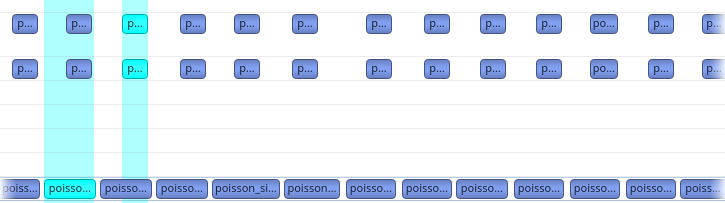
\includegraphics[width=\textwidth]{Ch48Implementation/figures/cudagraphs_before.png}
        \caption{Before CUDA Graphs}
    \end{subfigure}
    \vspace{1cm}
    \begin{subfigure}{\textwidth}
        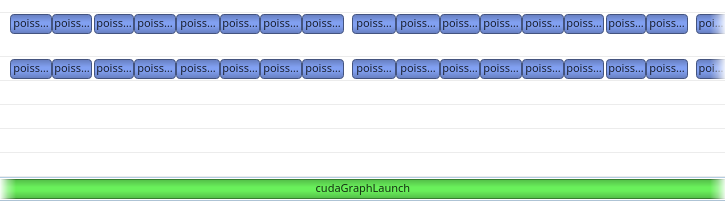
\includegraphics[width=\textwidth]{Ch48Implementation/figures/cudagraphs_after.png}
        \caption{After CUDA Graphs}
    \end{subfigure}
    \caption{Profiler traces of the Poisson kernels before and after CUDA graphs}
    \label{fig:CudaGraphsImpact}
\end{figure}

The timestep calculation is implemented with two reductions, implemented with the second kernel from \cite{CUDAParallelReduction}\footnote{This isn't the fastest kernel, but reductions aren't frequent enough for it to matter.}.
A constant factor N is chosen, and the values in the array are reduced by a factor of N multiple times until only one is left.
Two data buffers are used to ping-pong the reductions - each iteration flips the input and output, so data is reduced from A to B to A and so on.

Because there are two reductions, it is most efficient to perform the first one asynchronously and enqueue both before waiting for them to finish.
By default copying reduction results back to the CPU is synchronous, which prevents this.
Allocating pinned memory, which cannot be paged to disk or moved around by the OS, allows the copy to be done asynchronously.

\begin{figure}
    \centering
    \subcaptionbox[0.49\linewidth]{Synchronous Copy}{%
        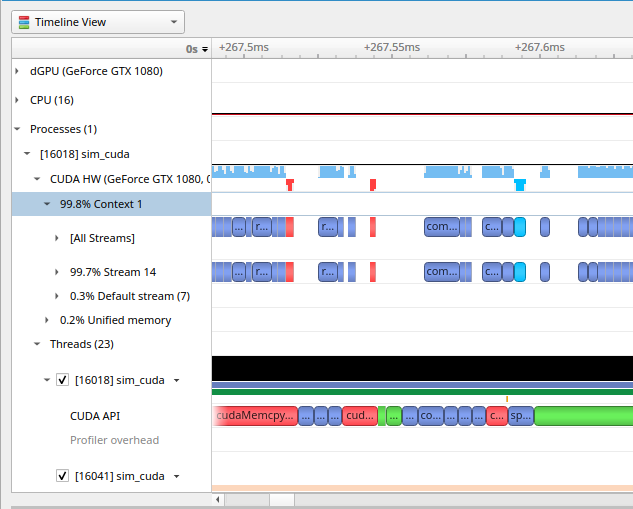
\includegraphics[width=\linewidth]{Ch48Implementation/figures/memcpy_sync.png}%
    }%
    \subcaptionbox[0.49\linewidth]{Asynchronous Copy}{%
        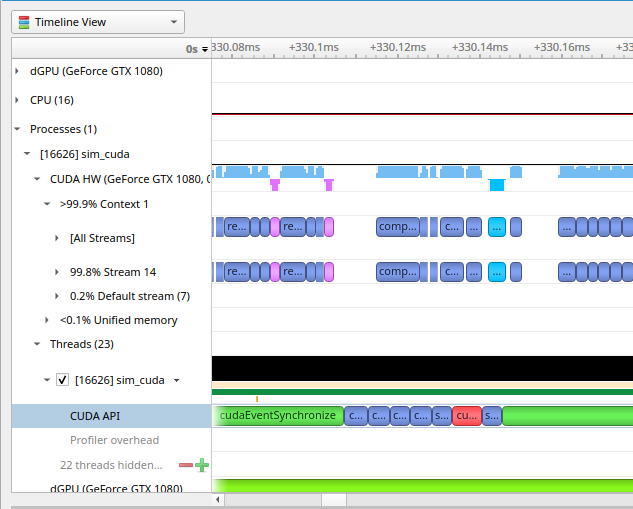
\includegraphics[width=\linewidth]{Ch48Implementation/figures/memcpy_async.png}%
    }% 
    \caption{Using asynchronous copies for greater efficiency}
    \label{fig:async_copy}
\end{figure}

% Copying the result back to the CPU is done asynchronously, which requires pinned memory to be allocated\todocite{pinned memory}.
% Normal virtual memory can be paged to disk or moved around by the OS, which means there is no reliable location for the GPU to eventually copy data to.
% Pinned memory must be specially allocated, and cannot be moved around, so the asynchronous copy can go ahead as planned.
% If pinned memory were not used the copy to CPU would be synchronous, which would delay the second 

% The profiler showed X when not using pinned memory, as copies to non-pinned CPU memory are synchronous so must wait for the first reduction before enqueueing the second.

% Currently the CUDA program uses the second kernel model, and this is planned to be moved up to the seventh kernel in the future.

% The CUDA program uses the second kernel model. 
% Upgrading to the seventh model was considered, but as the program does not include the residual check, the reductions are infrequent enough (two per tick) that upgrading was not necessary.
% In the future, this may be improved if Poisson residuals were introduced.\todomark{actual future work}
% \todomark{Mention pinned memory here}

\subsection{Usage in Other Layers}
The visualization layer instantiates a \mintinline{cpp}{VulkanTickedRunner} with \mintinline{cpp}{CudaBackendV1} to run a visualized simulation.

The command-line layer instantiates a \mintinline{cpp}{FixedTimeRunner} with any one of the backends to run a headless simulation.